\documentclass[a4paper, 11pt]{article}
\usepackage{comment} 
\usepackage{lipsum} 
\usepackage{fullpage}
\usepackage{graphicx}
\usepackage{wrapfig}
\graphicspath{ {Images/} }
\setlength{\parskip}{1em}

\begin{document}
\noindent
\large\textbf{Amazon Reviews} \\
\textbf{Final Case Report} \\
\normalsize Professor Mittal \\
Jacob Mannix\hfill December 17th, 2019 \\
 
%%%%%%%%%%%%%%%%%%%%%%%%%%%%%%%%%%%%%%%%%%%%%%%%%%%%%%%%%%%%%%%%
\section*{Method and Process}

\begin{figure}[h]
  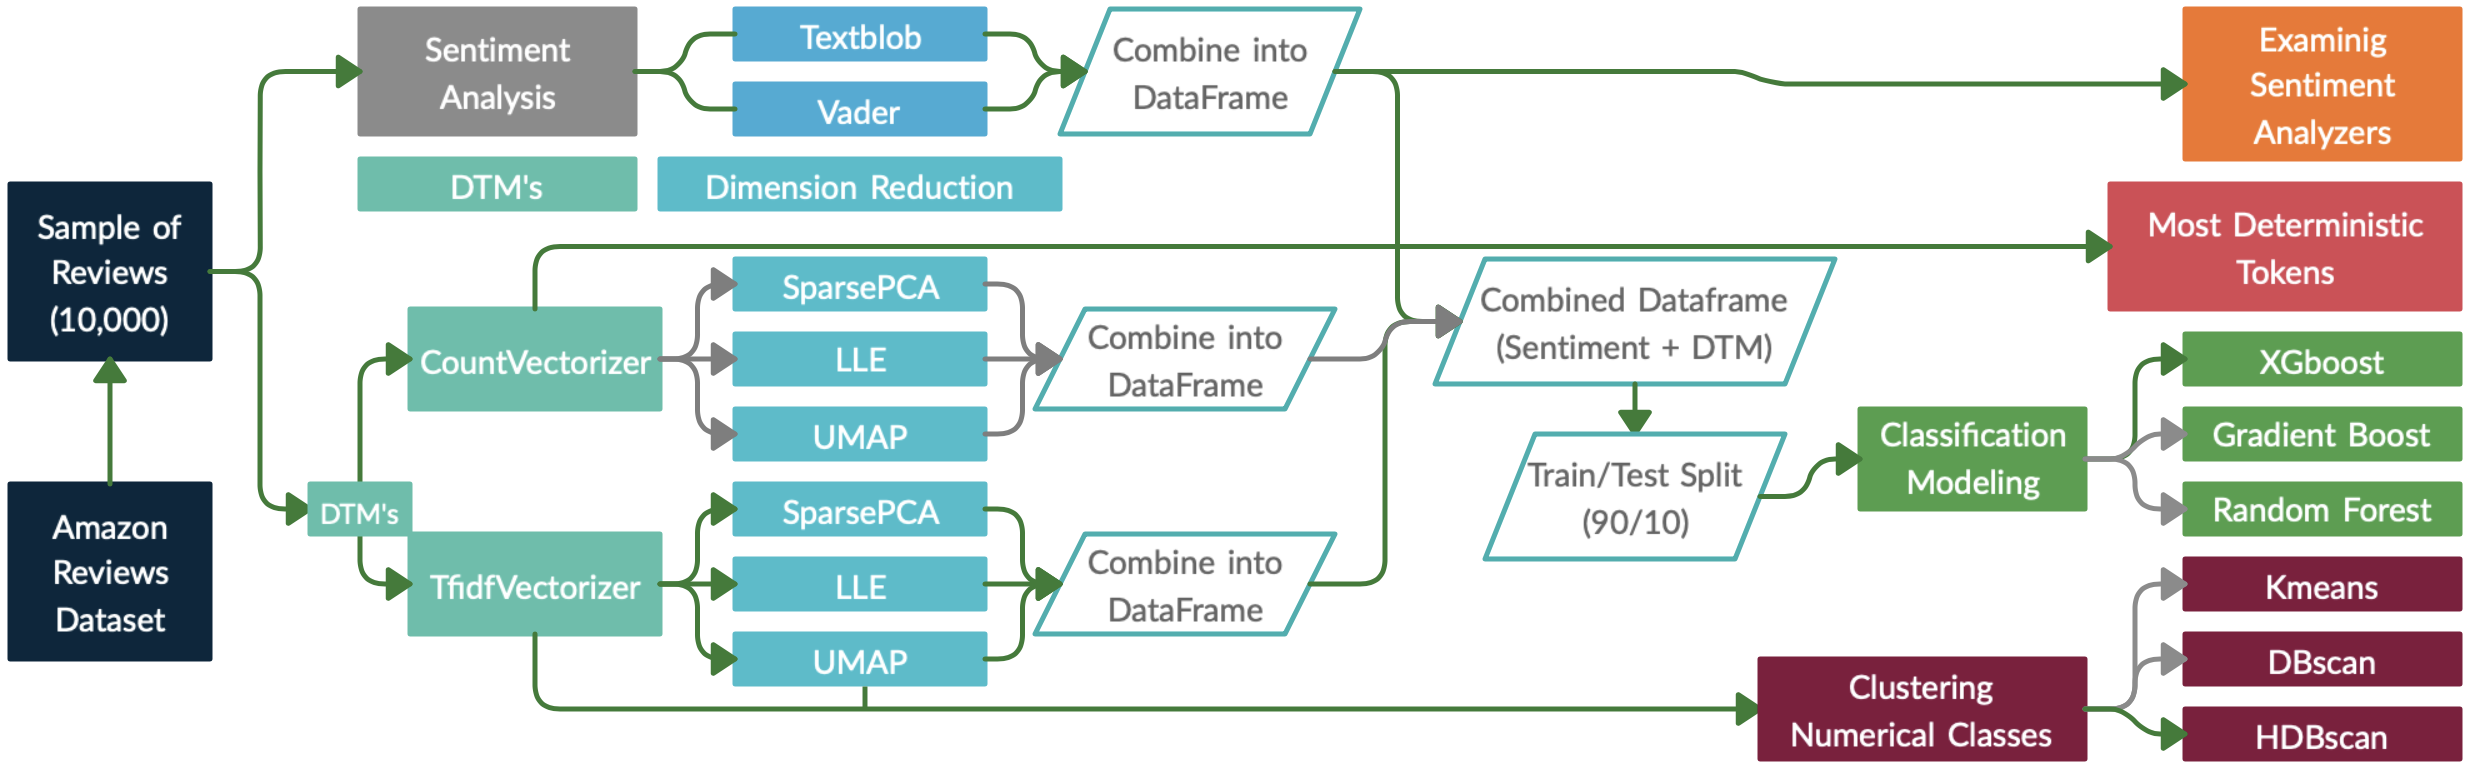
\includegraphics[width=\linewidth]{tree}
  %\caption{A boat.}
  %\label{fig:boat1}
\end{figure}
\noindent
The data set given was three million Amazon reviews with their respective rating, title and description spanning over eighteen years. The flow chart above outlines the process that I went through for this analysis. To begin on the left side, I created a sample of the full data set due to computing time.  I chose to take a sample of 10,000 rows. Each color indicates a different aspect of the process and green arrows indicates the preferred method over others. On the far right there are four colors indicating the four main sections which will be explaining more in detail below.

%%%%%%%%%%%%%%%%%%%%%%%%%%%%%%%%%%%%%%%%%%%%%%%%%%%%%%%%%%%%%%%%
\begin{wrapfigure}{r}{0.45\textwidth} %this figure will be at the right
    \vspace{7mm}
    \centering
    \caption{TextBlob}
    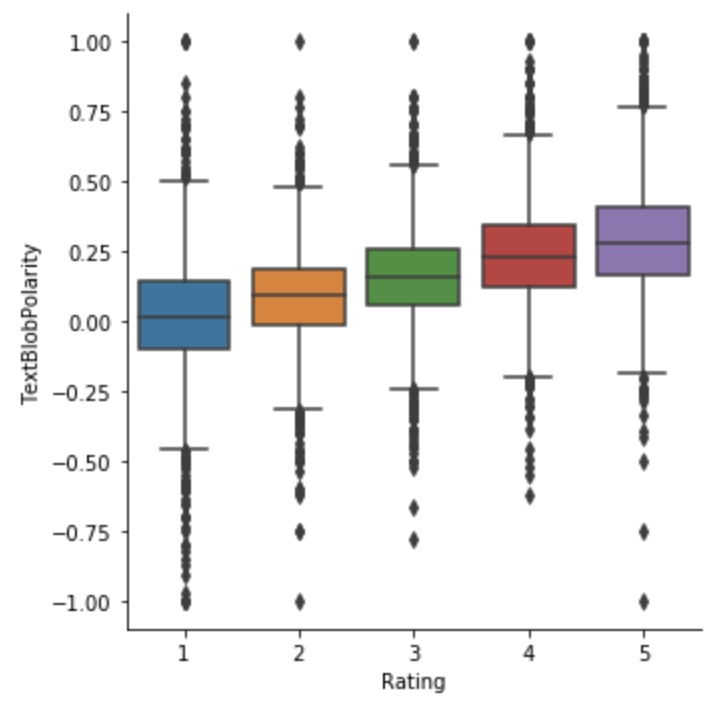
\includegraphics[width=\linewidth, trim=1 1 1 1,clip]{SentimentTextBlob.png}
\end{wrapfigure}

\section*{Examining Sentiment Analyzers}
To examine the quality of the sentiment analyzers, \emph{TextBlob} and \emph{Vader} I graphed the polarity scores along with the actual ratings of the reviews in order to see how accurate they were. 

\noindent
\emph{Figure 1} to the right showcases rating versus polarity score for \emph{TextBlob}. As shown in the graph it appears that on average when a review has a higher rating it has a more positive polarity score and when a review has a lower rating the polarity score is lower. That being said, the majority of the polarity scores seem to be between 0 and 0.5 with a few reaching the opposing peaks. As a whole \emph{TextBlob} seem to be fairly conservative in the ratings and chooses to score many of the reviews slightly above or below zero.

\begin{wrapfigure}{r}{0.45\textwidth} %this figure will be at the right
    \vspace{-3mm}
    \centering
    \caption{Vader}
    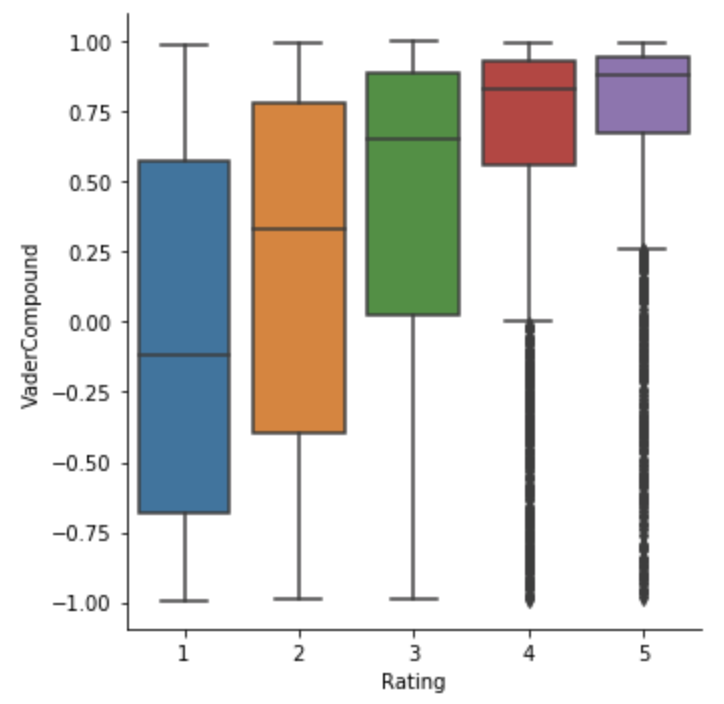
\includegraphics[width=\linewidth, trim=1 -35 1 -20,clip]{SentimentVader.png}
    \vspace{-20mm}
\end{wrapfigure}


\noindent
\emph{Figure 2} shown to the right displays the rating versus polarity scores for \emph{Vader}. As shown in the graph there is a noticeable distinction between polarity scores for each rating. The majority fifty percent of the box-plot spans a large range for a rating of one but becomes much smaller as the ratings increase. I think this could be due to \emph{Vader} not being as harsh on negative words/reviews that do not contain many negative words. This causes \emph{Vader} to do a pretty good job of separating reviews by polarity scores with higher ratings but struggles a bit with lower ratings.

\noindent
Overall, the two sentiment analyzers were able to partly distinguish ratings based off of their polarity scores, but they were by no means excellent. I think that between the two, \emph{Vader} did a better job than \emph{TextBlob} by being able to separate the difference in the ratings more being able to separate the majority of the four and five star ratings from the others.

%%%%%%%%%%%%%%%%%%%%%%%%%%%%%%%%%%%%%%%%%%%%%%%%%%%%%%%%%%%%%%%%
\section*{Classification Modeling}
To begin modeling I created a document term matrix using \emph{Tfidf Vectorizer} L2 parameters. I then ran for \emph{SparsePCA}, \emph{LLE} and \emph{UMAP} on the document term matrix to reduce the dimensions and combined these dimension reduced columns from \emph{SparsePCA}, \emph{LLE} and \emph{UMAP} together into one data frame. Next I added the polarity scores from \emph{Textblob} and \emph{Vader} to that data frame. After creating this combined data frame, I created a train/test split of 90/10. I chose this split because it was only a sample of 10,000 and I wanted to make sure I had a large enough set to train on. I chose to model using \emph{XGboost}, \emph{Gradient Boosting} and \emph{Random Forest}. I used \emph{GridSearchCV} to test a variety of hyper-parameters for each algorithm. After running many models, I ended with a best model \emph{Gradient Boosting} that predicted the numerical class with a \emph{38.9\%} accuracy score. For that best accuracy score I used a \emph{learning rate} of 0.01, 1000 \emph{estimators} and a \emph{sub-sample} of 0.4.

%%%%%%%%%%%%%%%%%%%%%%%%%%%%%%%%%%%%%%%%%%%%%%%%%%%%%%%%%%%%%%%%
\begin{wrapfigure}{r}{0.3\textwidth} %this figure will be at the right
    \centering
    \vspace{3mm}
    \caption{Kmeans}
    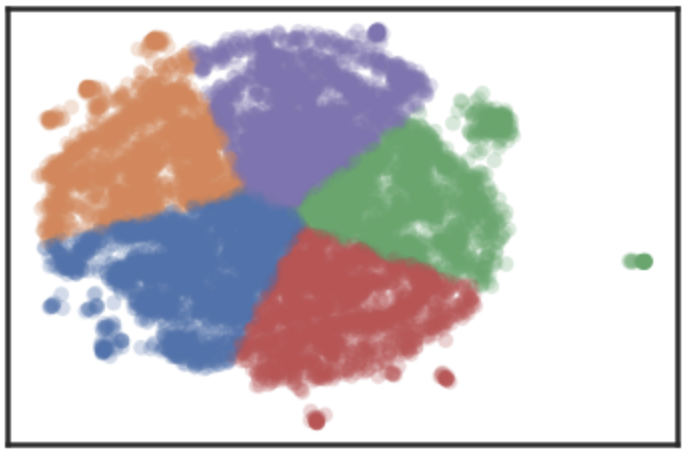
\includegraphics[width=\linewidth, trim=1 0 1 0,clip]{clusterkmeans.png}
\end{wrapfigure}

\section*{Clustering Numerical Classes}
\vspace{-1mm}
For clustering, I created a document term matrix created using \emph{Tfidf Vectorizer} and used \emph{UMAP} to reduce dimensions. I then clustered using \emph{Kmeans}, \emph{DBSCAN} and \emph{HDBSCAN}. Beginning with \emph{Kmeans}, shown in \emph{Figure 3} on the right with clusters separated by color, I tried a variety of different number of cluster sizes and could not find much evidence of separation within the rating classes. As seen in the figure there are clearly clusters but the distribution of ratings within each cluster are almost equal.

\begin{wrapfigure}{r}{0.3\textwidth} %this figure will be at the right
    \centering
    \vspace{-4mm}
    \caption{DBSCAN}
    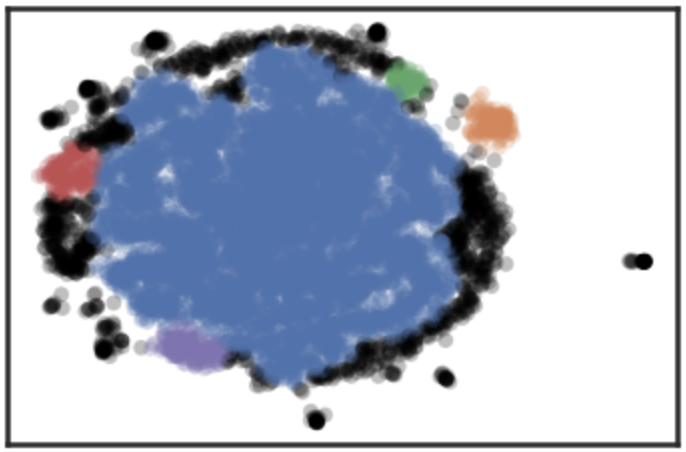
\includegraphics[width=\linewidth, trim=1 0 1 0,clip]{clusterdbscan.png}
    \vspace{-3mm}
    \caption{HDBSCAN}
    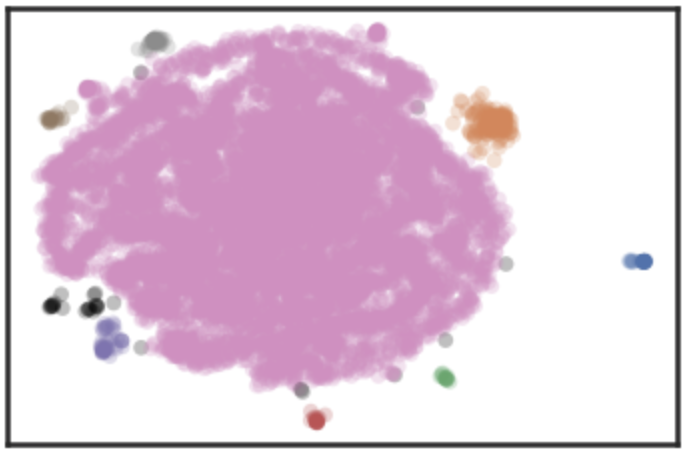
\includegraphics[width=\linewidth, trim=1 0 1 0,clip]{clusterhdbscan.png}
    % \vspace{-2mm}
\end{wrapfigure}

\noindent
As for \emph{DBSCAN}, there was not much evidence either. \emph{Figure 4} shown on the right, colored by cluster, shows a large cluster in the center with smaller clusters around the edges. I tried a variety of different sample sizes and none of them seemed to be able to separate the clusters based on the rating class. Similar to \emph{Kmeans} the clusters nearly equally distributed the rating classes.

\noindent
Lastly, \emph{HDBSCAN} was able to separate the data into more clusters than the previous two options but these additional clusters did not offer much in revealing the rating class. As seen in \emph{Figure 5} on the right, there is a large cluster in the center, similar to \emph{DBSCAN} but there are many more smaller clusters around the edges. Once again these clusters were fairly equally distributed throughout all of the rating classes. 

\noindent
Overall, I do not think that clustering alone is a good method to identify the rating class. The methods specified above did not offer much of anything in trying to reveal the differences in rating classes. 

%%%%%%%%%%%%%%%%%%%%%%%%%%%%%%%%%%%%%%%%%%%%%%%%%%%%%%%%%%%%%%%%
\section*{Most Deterministic Tokens}
\noindent
In order to try and determine the most deterministic tokens for each rating I decided use the \emph{CountVectorizer} document term matrix. I converted this to a data frame and created a pivot table of the data in order to see the percent of a specific word in each of the numerical classes for ratings. I then took the top 50 most used words for each class and compared them. There were many duplicates and I wanted to remove some to get a better understanding so I decided to remove them but did not remove duplicate words for classes that were adjacent to one another (i.e. For a rating of 2, not removing duplicates that came from rating 1 and 3). I did this because many words were used in all rating classes and I thought this would give a better look into the main differences between good and bad reviews. Also, if the top word is in all classes then it is not very deterministic of the rating if they all have it. By doing this I end up with lists of most used words for each rating class of around 5-10 words in length. 

\begin{figure}[h]
  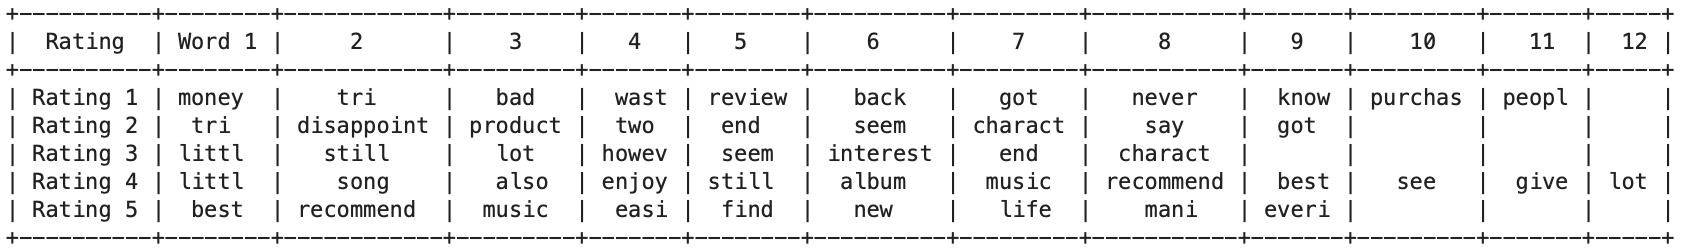
\includegraphics[width=\linewidth]{DetermTokens1.png}
  %\caption{A boat.}
  %\label{fig:boat1}
\end{figure}

\noindent
After looking at the different words in each of the classes it is understandable as to why many of these words are present from some rating classes and absent from others. For instance, also seen in the figure above, the words \emph{‘best’} and \emph{‘recommend’} are at the top of the list for a rating of five and the words \emph{‘bad’} and \emph{‘wast’} are near the top of the list for a rating of one. One word that surprised me was \emph{‘money’}. I would have thought \emph{‘money’} would be fairly evenly distributed through all classes, but it appeared as the top word for rating one.

\end{document}